\documentclass[11pt, a4paper]{article}

\usepackage[utf8]{inputenc}
\usepackage[T1]{fontenc}
\usepackage{amsmath, amssymb}
\usepackage{graphicx}
\usepackage[hidelinks]{hyperref}
\usepackage{booktabs}
\usepackage{geometry}
\geometry{margin=1in}

\title{\textbf{Kalpana-RIF Discrete: Neuro-Symbolic Reranking of Code-Search Candidates for Agentic Retrieval Pipelines}}
\author{Madusha \\ Takara/Miru Research}
\date{\today}

\begin{document}

\maketitle

\begin{abstract}
Coding agents that retrieve code chunks for an LLM face a trade-off: a larger candidate list raises the chance that the defining chunk is present, but it also adds distractor context. We study \emph{Kalpana-RIF Discrete}, a small structural reranker placed behind Miru's native hybrid retriever. It binds tree-sitter identifier roles (function, argument, class, variable, call) to mean-centred token embeddings using FFT-based circular convolution, scores the retriever's top-5 candidates by cosine similarity, and fuses that score with the native score (RRF, or a linear blend with weight chosen by cross-validation). The goal is to keep in the top 3 what the native top 5 would have contained.

On held-out sets, Kalpana's top 3 retains about 97\% of the chunks that the native top 5 contains, versus about 83\% for the native top 3, on two large sets (identifier-style and docstring-style queries). On 1,853 identifier queries over 14 repositories, top-3 chunk accuracy rises from 51.2\% to 59.5\% (168 wins, 15 losses, $p<0.001$) against a top-5 ceiling of 61.3\%. Gains are smaller on CodeSearchNet (73.3\% $\to$ 75.5\%) and on a 500-query \texttt{client-go} set with a MiniLM codebook (54.8\% $\to$ 59.8\%). Scoring a 5-chunk pool takes about 0.05\,ms; building a query tensor costs one extra embedding call unless it is cached. All results are retrieval metrics: we pass 40\% fewer chunks (3 instead of 5) but have not evaluated downstream LLM answer quality. We list the limitations, including shared parsers between labels and features and one repository per language, in Section~\ref{sec:limits}.
\end{abstract}

\section{Introduction}
Retrieval-augmented coding assistants must decide how many retrieved chunks to place in the model's context. Code is relational: whether a chunk \emph{defines} a function, merely \emph{calls} it, or only mentions its name depends on syntactic structure that a single dense vector represents only implicitly. Native Miru uses hybrid (dense plus lexical) retrieval, which has strong recall in its top 5 but a noticeably lower top-3 hit rate. This leaves a gap between ``the right chunk is in the pool'' and ``the right chunk is in the context we can afford''.

We address that gap with a reranker that does not replace the retriever. Kalpana-RIF Discrete only reorders Miru's top-5 pool, so its attainable accuracy is bounded by the pool's recall (the \emph{top-5 ceiling}). The question we ask is how much of that ceiling can be retained with only 3 chunks.

An earlier continuous variant of our engine, based on additive superposition with time-based wave modulation, was found in our own experiments to be less suited to this task because summed embeddings blur role information. We do not rely on that observation here and make no claim about transformer embeddings in general; the present paper evaluates only the discrete variant.

\section{Method}
\begin{figure}[h]
\centering
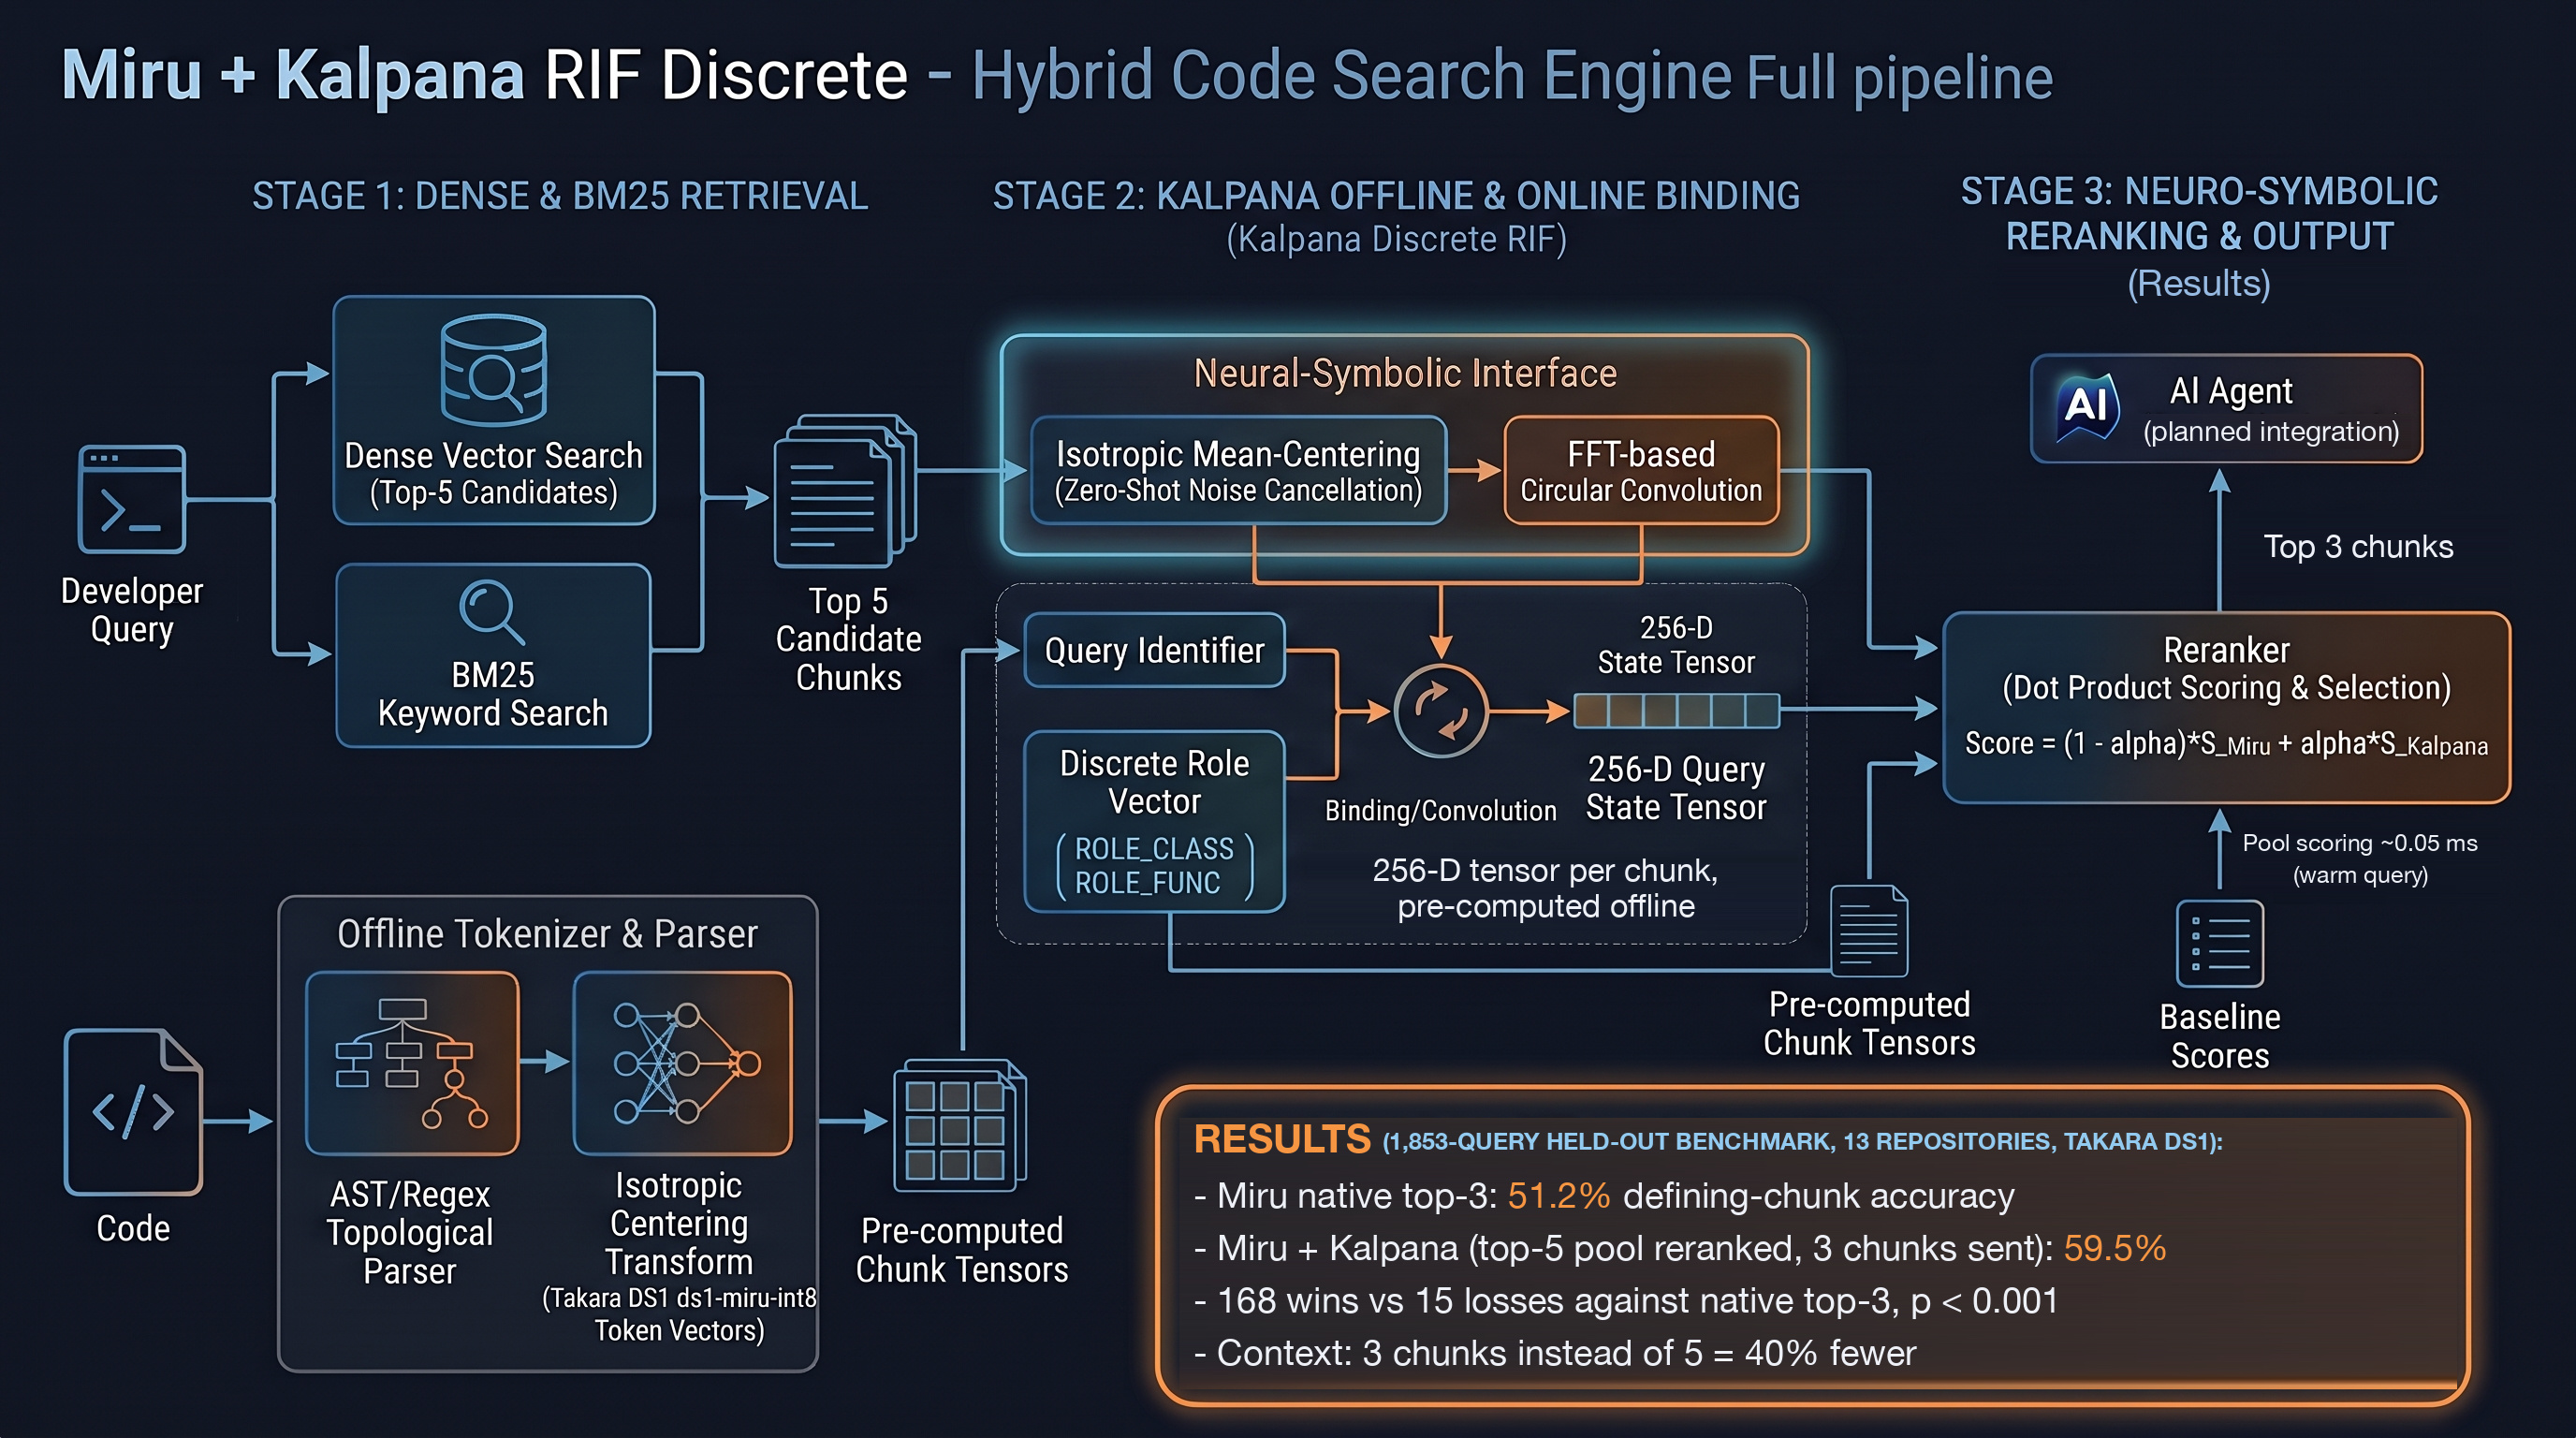
\includegraphics[width=\linewidth]{../docs/architecture.jpeg}
\caption{Pipeline overview: Miru retrieves a top-5 pool; Kalpana-RIF builds a role-bound tensor per candidate, scores it against a query tensor, and fuses the two rankings into a top-3.}
\end{figure}

\subsection{Role extraction}
For each candidate chunk we run tree-sitter and extract (role, identifier) pairs for five roles: \texttt{ROLE\_FUNC}, \texttt{ROLE\_ARG}, \texttt{ROLE\_CLASS}, \texttt{ROLE\_VAR} and \texttt{ROLE\_CALL}.

\subsection{Role vectors and token vectors}
Each role $r$ has a fixed, deterministic random \emph{unitary} vector $\mathbf{r}$ (FFT phases random, all magnitudes 1, seeded by a hash of the seed and role name). Unitary vectors make circular-convolution binding norm-preserving and invertible. Each identifier token $t$ is embedded with the retriever's embedding model and mean-centred against a reference set of words:
\begin{equation}
\mathbf{x}_t = \frac{\mathrm{embed}(t) - \bar{\mathbf{e}}}{\lVert \mathrm{embed}(t) - \bar{\mathbf{e}} \rVert},
\end{equation}
where $\bar{\mathbf{e}}$ is the mean embedding of the reference words. Mean-centring removes the shared component that makes all embeddings look mutually similar; it does not make distinct tokens orthogonal. The embedding dimension is 256 for the DS1 codebook and 384 for MiniLM.

\subsection{Binding and scoring}
Binding is circular convolution, computed with FFTs. The tensor of a chunk with pairs $\{(r_i, t_i)\}$ is
\begin{equation}
\mathbf{T}_{\text{chunk}} = \sum_i \mathbf{r}_i \circledast \mathbf{x}_{t_i}.
\end{equation}
It has the same fixed dimension $d$ regardless of the chunk length. For a query $q$ we form
\begin{equation}
\mathbf{T}_{q} = \mathbf{r}_{\text{FUNC}} \circledast \mathbf{x}_q + \mathbf{r}_{\text{CLASS}} \circledast \mathbf{x}_q,
\end{equation}
so a query is matched against chunks that hold the query's name in a function or class role. The Kalpana score is the cosine similarity $\cos(\mathbf{T}_q, \mathbf{T}_{\text{chunk}})$. Scoring a pool is linear in the pool size.

\subsection{Fusion}
We fuse the Miru ranking and the Kalpana ranking in one of two ways: reciprocal rank fusion (RRF), or a linear blend
\begin{equation}
s = (1-\alpha)\,\mathrm{minmax}(s_{\text{Miru}}) + \alpha\,\mathrm{minmax}(s_{\text{Kalpana}}),
\end{equation}
with $\alpha$ chosen by 5-fold cross-validation and every reported number scored on the held-out fold only.

\section{Evaluation}
\subsection{Setup and metrics}
A query counts as a hit at 3 if the chunk that defines the target symbol is among the top 3 returned. \emph{Native} is Miru's own top 3; \emph{Kalpana} is the fused reranking of Miru's top 5. We report wins and losses (queries where only one system hits) and two-sided exact sign-test $p$-values. We give two comparisons: against the native top 3 (the practical comparison) and against the \emph{same top-5 pool} (the controlled comparison, which isolates the reranking). The \emph{top-5 ceiling} is the fraction of queries whose target is in the native top 5.

\subsection{\texttt{client-go}, 500 queries (MiniLM codebook, RRF)}
The first 150 queries were used during development. The remaining 350 were generated after the method was fixed and the primary test was set before they were run, so we treat them as confirmatory.

\begin{table}[h]
\centering
\begin{tabular}{@{}lccc@{}}
\toprule
 & \textbf{Native top-3} & \textbf{Kalpana top-3} & \textbf{Gain} \\ \midrule
File@3, all 500 & 82.4\% & 85.8\% & +3.4 \\
Chunk@3, all 500 & 54.8\% & 59.8\% & +5.0 \\
Chunk@3, new 350 only & 56.9\% & 62.3\% & +5.4 \\ \bottomrule
\end{tabular}
\caption{\texttt{client-go}. All rows are on the same query set as their label states; Chunk@3 top-5 ceiling is 64.6\%.}
\end{table}

Against the native top 3, Chunk@3 has 32 wins and 7 losses ($p=0.0001$) and File@3 has 24 wins and 7 losses ($p=0.003$). Against the same top-5 pool, Chunk@3 has 32 wins and 1 loss ($p=7.9\times10^{-9}$) and File@3 has 28 wins and 4 losses ($p=1.9\times10^{-5}$). On the confirmatory 350 queries alone: 23 wins, 4 losses, $p=0.0003$. Kalpana's 59.8\% is 92.6\% of the 64.6\% ceiling; it does not exceed it.

\subsection{Multi-language results (DS1 codebook)}
These runs use the DS1 embedder both as Miru's retriever and as Kalpana's codebook (see limitations).

\begin{table}[h]
\centering
\small
\begin{tabular}{@{}lrcccc@{}}
\toprule
\textbf{Suite} & $n$ & \textbf{Native} & \textbf{Kalpana} & \textbf{W / L} & \textbf{Top-5 ceiling} \\ \midrule
CodeSearchNet, 6 languages & 3,000 & 73.3\% & 75.5\% & 93 / 27 & 77.9\% \\
Identifier, tree-sitter labels & 1,853 & 51.2\% & 59.5\% & 168 / 15 & 61.3\% \\
Identifier, independent labels & 1,853 & 57.4\% & 63.6\% & 145 / 30 & --- \\
Docstring-style, 8 languages & 1,537 & 27.9\% & 32.5\% & 80 / 10 & $\approx$33.4\% \\ \bottomrule
\end{tabular}
\caption{Chunk@3, native top-3 versus Kalpana top-3 (fused, $\alpha$ by 5-fold CV). Win/loss is against the native top 3; all four $p<0.001$.}
\end{table}

Against the same top-5 pool, the win/loss counts are 81/24 (CodeSearchNet), 181/12 (identifier) and 75/5 (docstring-style). With a MiniLM codebook, CodeSearchNet was a smaller and non-significant change (74.6\% $\to$ 75.3\%, 64/43, $p=0.053$). The \emph{independent-label} row re-labels the identifier targets using Pygments lexers and regexes instead of tree-sitter, to test whether the gain depends on the labeller sharing a parser with the features.

\paragraph{Docstring-style queries.} These queries are paraphrased from docstrings rather than copied identifiers. On the 1,186 queries with no identifier-word overlap with the target the gain is 25.2\% $\to$ 29.3\% (56 wins, 7 losses); on the 351 queries containing all identifier words it is 37.0\% $\to$ 43.0\% (24/3). File@3 changes from 61.3\% to 64.1\% (101/58), a much weaker effect than at chunk level.

\subsection{Share of the top-5 ceiling retained}
Because Kalpana can only reorder Miru's pool, a natural summary is how much of the pool's hits survive when cut to 3 chunks:

\begin{table}[h]
\centering
\begin{tabular}{@{}lcc@{}}
\toprule
\textbf{Suite} & \textbf{Native top-3 / top-5} & \textbf{Kalpana top-3 / top-5} \\ \midrule
Identifier (DS1) & 83\% & 97\% \\
Docstring-style (DS1) & 83\% & 97\% \\
CodeSearchNet (DS1) & 94\% & 97\% \\
\texttt{client-go} (MiniLM) & 85\% & 93\% \\ \bottomrule
\end{tabular}
\caption{Share of top-5 ceiling retained by the top 3 chunks.}
\end{table}

This is \emph{not} accuracy and it is not 97\% on every suite. It is also not lossless: even against the same pool, the reranker loses a small number of queries relative to that pool (for example 1 of 500 on \texttt{client-go} and 12 of 1,853 on the identifier suite). The attainable gain is limited by the retriever's pool.

\subsection{Latency}
Latencies below are median (p50) wall times for DS1.

\begin{table}[h]
\centering
\begin{tabular}{@{}lr@{}}
\toprule
\textbf{Step} & \textbf{p50 (ms)} \\ \midrule
Miru query embedding & 121--131 \\
Miru search & 5--46 \\
Kalpana query tensor, warm (cached embedding) & 0.2 \\
Kalpana pool scoring (5 chunks) & 0.05 \\
Kalpana query tensor, cold (own embedding call) & 353--370 \\ \bottomrule
\end{tabular}
\caption{Latency including query embedding. With MiniLM on CPU, the \texttt{client-go} runs measured 0.035\,ms p50 (0.055\,ms p95) for pool scoring and 9.3\,ms per new query encode.}
\end{table}

Pool scoring is sub-millisecond; an uncached query is not, because the query must be embedded. Reusing Miru's query vector would remove the cold cost but is not yet implemented.

\section{Limitations and Future Work}\label{sec:limits}
\begin{itemize}
\item \textbf{Shared parser.} Chunk features and the tree-sitter labels use the same parser. The independent-label run reduces but does not eliminate this concern.
\item \textbf{One repository per language,} and several small sets (C 43, C++ 57, Elixir 28, TypeScript 47, Haskell 78 queries), so per-language numbers are noisy.
\item \textbf{DS1 plays two roles}: it is Miru's retriever and Kalpana's codebook. An ablation separating the two has not been run.
\item \textbf{Coverage.} Solidity and OCaml are not indexed by Miru (no extension mapping); Dart's grammar does not load in the tree-sitter build used; Bash, SQL and markup languages were not evaluated.
\item \textbf{Retrieval metrics only.} We counted chunks, not tokens or KV-cache size, and did not evaluate downstream LLM or agent quality. ``40\% fewer chunks'' is a statement about chunk count.
\item \textbf{Missing baselines and ablations.} We have not compared against a lexical or regex reranker, a cross-encoder, or a ``bundle plain sum without binding'' ablation. These are future work.
\item \textbf{Headline run uses MiniLM.} The 500-query \texttt{client-go} run has not been repeated with the DS1 codebook.
\end{itemize}

\section{Reproducibility}
Code, scripts, query sets and pinned data are available in the repository \url{https://github.com/maduperera/Miru_Discrete_RIF}. Role vectors are seeded deterministically; the DS1 API key is read from the environment and is not stored in the repository. Evaluation scripts include the fusion benchmark, the independent re-labelling script and the docstring-suite runner described in the README.

\section{Conclusion}
Kalpana-RIF Discrete is a lightweight reranker that binds tree-sitter identifier roles to token embeddings and reorders Miru's top-5 pool. On held-out identifier-style and docstring-style sets it lets 3 chunks keep about 97\% of the hits that 5 chunks would, compared with about 83\% for the native top 3, with significant win/loss margins ($p<0.001$). Gains are modest on natural-language-style retrieval and are bounded by the retriever's pool. Pool scoring is cheap, but a cold query adds an embedding call. Whether the smaller context improves agent behaviour remains to be measured.

\end{document}
